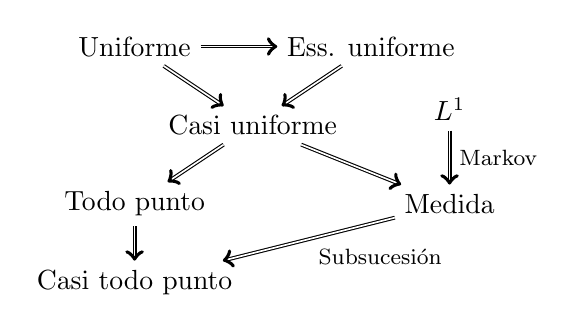
\begin{tikzpicture}
\node (U) at (0,4) {Uniforme};
\node (EU) at (3,4) {Ess. uniforme};
\node (CU) at (1.5,3) {Casi uniforme};
\node (TP) at (0,2) {Todo punto};
\node (CTP) at (0,1) {Casi todo punto};
\node (L1) at (4,3.2) {$L^1$};
\node (MED) at (4,2) {Medida};

\draw[->, double] (U) -- (EU);
\draw[->, double] (U) -- (CU);
\draw[->, double] (EU) -- (CU);
\draw[->, double] (CU) -- (TP);
\draw[->, double] (TP) -- (CTP);
\draw[->, double] (L1) -- node[midway, right] {\footnotesize Markov} (MED);
\draw[->, double] (CU) -- (MED);
\draw[->, double] (MED) -- node [midway, below right] {\footnotesize Subsucesión} (CTP);
\end{tikzpicture}
